% arXiv: primary cs.AI; cross-list cs.SE, cs.PL
% Comments: operational semantics for tool-using agent loops; four conformant
% kernels (CPython, POSIX sh, SQL, ARM64 assembly); conformance, ablation,
% equivalence, fault-injection and systems measurements
\documentclass[11pt,a4paper]{article}
\usepackage[margin=1in]{geometry}
\usepackage{times}
\usepackage{hyperref}
\usepackage{booktabs}
\usepackage{amsmath}
\usepackage{url}
\usepackage{graphicx}
\usepackage[T1]{fontenc}
\usepackage[utf8]{inputenc}

%% generated by alm/paper_tables.py -- do not edit
\newcommand{\adapterloc}{343}
\newcommand{\almfields}{13}
\newcommand{\almrules}{9}
\newcommand{\confcases}{350}
\newcommand{\confdisagree}{0}
\newcommand{\confruns}{700}
\newcommand{\confwall}{2.4}
\newcommand{\containerplatform}{Linux x86\_64}
\newcommand{\containerpython}{3.13.12}
\newcommand{\containerruns}{1050}
\newcommand{\containersqlite}{3.40.1}
\newcommand{\faultdup}{0}
\newcommand{\faultredelivered}{14288}
\newcommand{\fullclean}{1.000}
\newcommand{\fullfifty}{0.520}
\newcommand{\fullten}{1.000}
\newcommand{\livecapped}{357}
\newcommand{\liveruns}{3440}
\newcommand{\localmaxdiff}{0.015}
\newcommand{\localn}{1920}
\newcommand{\localpassk}{5}
\newcommand{\localreps}{5}
\newcommand{\localtasks}{24}
\newcommand{\modeldiff}{-0.234}
\newcommand{\modeldiffnt}{-0.164}
\newcommand{\modelratio}{4}
\newcommand{\modelshare}{98.8\%}
\newcommand{\modeltimeouts}{29}
\newcommand{\mutcaught}{17}
\newcommand{\mutmin}{10}
\newcommand{\muttotal}{17}
\newcommand{\nmodels}{4}
\newcommand{\norecclean}{1.000}
\newcommand{\norecten}{0.720}
\newcommand{\oracleetaarm}{0.869}
\newcommand{\oracleetafamily}{0.005}
\newcommand{\oracleetakernel}{0.000}
\newcommand{\orchshare}{0.13\%}
\newcommand{\recoverygain}{28}
\newcommand{\slowestshare}{0.71}
\newcommand{\slowestus}{3561}
\newcommand{\submaxdiff}{0.000}
\newcommand{\subreps}{3}
\newcommand{\subruns}{2400}
\newcommand{\tbagentfault}{23}
\newcommand{\tbarmone}{0.171}
\newcommand{\tbarmtrials}{801}
\newcommand{\tbarmtwo}{0.465}
\newcommand{\tbdifferent}{0}
\newcommand{\tbdisagree}{37}
\newcommand{\tbequiv}{0}
\newcommand{\tbeveryone}{21}
\newcommand{\tbexcluded}{10}
\newcommand{\tbexcludedfirstrep}{1}
\newcommand{\tbinconclusive}{3}
\newcommand{\tbmaxdiff}{0.052}
\newcommand{\tbpromptdiff}{+0.028}
\newcommand{\tbreps}{1}
\newcommand{\tbsomeone}{62}
\newcommand{\tbtasks}{89}
\newcommand{\tbtrials}{2461}
\newcommand{\tcbspread}{196}
\newcommand{\throughputspread}{1656}


% Tables generated from results files are wide; scale rather than overflow.
\newcommand{\widetable}[1]{\resizebox{\textwidth}{!}{\input{#1}}}
\emergencystretch=3em

\title{How Small Can an Agent Runtime Be?\\
       Substrate-Neutral Semantics for Tool-Using LLM Agents}
\author{
  Hao Li\\
  Institute of Chemistry, Chinese Academy of Sciences\\
  Beijing, China\\
  \texttt{leeehow@gmail.com}\\
  ORCID \texttt{0009-0004-2696-3267}\\
  \texttt{https://github.com/Leehow/seed}
}
\date{August 2026}

\begin{document}
\maketitle

\begin{abstract}
An LLM agent run is usually shipped as one program, but it is three functions:
a model $\mu$, an environment $\varepsilon$, and a kernel $\kappa$ that decides
what the model sees next, what the budget is, and when the run is over.
We specify $\kappa$ alone.
The Agent Loop Machine (ALM) is an operational semantics for finite-horizon,
single-agent, observation-dependent tool use, with one unusual normative rule:
the kernel is \emph{payload-blind}---prompt bytes, tool output and diff hunks
are named by opaque references it moves but never reads.
What is left is a transition table over small integers and short tokens.
We implement it four times on deliberately unlike substrates---CPython, POSIX
\texttt{/bin/sh}, SQL triggers, and ARM64 assembly---and test whether they are
the same machine rather than four similar programs.
On \confcases\ recorded conformance cases the four kernels produce
byte-identical canonical traces (\confdisagree\ disagreements over \confruns\
runs) and match a separately written, table-driven oracle record for record;
\mutcaught\ of \muttotal\ seeded semantic mutations of the reference kernel
are caught.
Holding $\mu$, $\varepsilon$, the prompt bytes and the budget fixed, per-task
success rates across the four substrates differ by at most \localmaxdiff\ on
graded shell work and \submaxdiff\ on a live stochastic suite, inside a
pre-registered $\pm5$\,pp equivalence band; on \tbarmtrials\ Terminal-Bench 2.1
trials under the official verifier the three container-capable substrates
differ by at most \tbmaxdiff, no pair judged different, and that largest
difference lives entirely in one of the three repeats. Swapping the model
for one from another vendor, with the kernel and everything else held byte
identical, moves the same measurement by \modeldiff---roughly \modelratio\
times as much as swapping the substrate does.
Ablations show what the core is for: removing observation feedback,
cross-step state, or the recursion collapses success on witness families built
so that no controller lacking that piece can be right on every instance, and
bounded repair and retry are worth nothing at fault rate $0$ but
$+\recoverygain$\,pp at $10\%$.
The four kernels span $\throughputspread\times$ in transition throughput and
$\tcbspread\times$ in trusted computing base, yet the slowest is
\slowestshare\% of one model call.
Orchestration substrate is operationally necessary and no longer
performance-dominant.
\end{abstract}

\section{Introduction}

Agent frameworks are large, and it is not obvious how much of that size is load
bearing. The usual way to ask is ablation inside one framework, which answers a
question about that framework. We ask a different one: what is the smallest
object that still deserves the name \emph{agent loop}, and does the machinery
that runs it change what the agent can do?

The question only becomes tractable after a separation. An agent run is
commonly written as one program, but it is three functions:

\begin{align}
a_t         &\sim \mu(\mathrm{serialize}(s_t)) \label{eq:mu}\\
(w_{t+1}, o_t) &= \varepsilon(w_t, a_t)        \label{eq:eps}\\
s_{t+1}     &= \kappa(s_t, a_t, o_t)           \label{eq:kappa}
\end{align}

$\mu$ is the model: stochastic, expensive, and where task competence lives.
$\varepsilon$ is the environment: a filesystem, processes, a network, and where
the work actually happens. $\kappa$ is the kernel: deterministic, cheap, and
the only part that is a \emph{runtime}. Frameworks bundle all three. This paper
specifies $\kappa$ and measures what happens when you keep it and change
everything about how it is built.

Our specification, ALM v0.1~\cite{almspec}, adds one rule that does most of the
work. A kernel is \textbf{payload-blind}: history entries are opaque references
minted by the adapter, and a kernel may move them but never read the bytes
behind them. Every decision a kernel makes---which step is next, whether the
budget is spent, whether an event is stale, whether the run is over---is then a
comparison between small integers and short tokens. That is a claim about agent
loops, not an implementation trick, and it has a testable consequence: the
semantics should fit in a substrate with no string library at all.

We implement ALM four times: a Python reference, a POSIX shell kernel that
never forks after start-up, a SQL kernel whose transitions are \texttt{WHERE}
clauses in database triggers, and an ARM64 assembly kernel using five
syscalls. They share one adapter---byte-identical, supplying $\mu$ and
$\varepsilon$---so that any difference between them is the kernel's.

\paragraph{Contributions.}
\begin{enumerate}
\item \textbf{A specification of $\kappa$ alone} (\S\ref{sec:alm}) with an
explicit claim boundary, a wire format narrow enough to parse by byte scan, and
a canonical trace that makes two kernels comparable in one hash.
\item \textbf{Four conformant kernels} (\S\ref{sec:kernels}) on substrates that
share almost nothing, and a \confcases-case conformance suite that is
mutation-tested so that passing it means something (\S\ref{sec:h1}).
\item \textbf{Necessity witnesses} (\S\ref{sec:h4}): four task families that
separate feedback, cross-step state, recursion and stopping, each reported
against an information-theoretic ceiling and against live models.
\item \textbf{Equivalence rather than absence of significance}
(\S\ref{sec:h2}): pre-registered $\pm5$\,pp bands, task-clustered bootstrap,
and a variance decomposition over a fully crossed
model$\times$substrate$\times$task design.
\item \textbf{A reliability surface} (\S\ref{sec:faults}) and a two-number
systems account---kernel-only footprint and trusted computing base---that does
not let an assembly kernel pretend libc is free (\S\ref{sec:systems}).
\end{enumerate}

\paragraph{What we do not claim.}
We do not claim ALM is the minimal core for agents in general. It is a
candidate minimal core for finite-horizon, single-agent, observation-dependent
tool use; multi-agent coordination, human-in-the-loop approval, long-lived
memory and real-time control are outside v0.1 by normative text, not by
oversight. We do not report a Terminal-Bench leaderboard rank. And we keep the
research kernels strictly separate from this repository's production runtime
(\S\ref{sec:seed}): a 120\,KB shell agent with a capability index, packs and a
memory system is not evidence about minimality, and calling it that would be
the first thing a reader should reject.

\section{Related work}

\paragraph{Agent loops as state machines.}
StateFlow models LLM task solving as state-driven workflows~\cite{wu2024stateflow},
and TapeAgents represents an agent's trajectory, state and resumption as one
append-only tape~\cite{bahdanau2024tapeagents}. Both establish that agent
behaviour is usefully described as state evolution. Neither asks whether the
state machine is portable across computational substrates, nor supplies a
conformance criterion by which two implementations could be judged the same
machine. That gap---semantics with a test, rather than an architecture---is
what \S\ref{sec:alm} and \S\ref{sec:h1} address.

\paragraph{Thin agents.}
Agentless argues that much agent scaffolding is unnecessary for software
repair~\cite{xia2024agentless}, and mini-SWE-agent shows a small bash-centric
loop remains competitive~\cite{minisweagent}. Quine realises agents as native
POSIX processes~\cite{quine2026}. These make the case that \emph{less
framework} suffices. They do not separate which reductions cost capability from
which cost only reliability; our ablations (\S\ref{sec:h4}) and fault surface
(\S\ref{sec:faults}) are aimed exactly at that split.

\paragraph{Agent--computer interfaces.}
SWE-agent shows that an interface designed for models beats a raw shell on
repository repair~\cite{yang2024sweagent,jimenez2024swebench}. We hold the
interface fixed at two primitives across every arm precisely because it is
known to matter: an experiment that varied the substrate and the tool surface
together would measure neither.

\paragraph{Benchmarks and reliability.}
Terminal-Bench evaluates long-horizon terminal work in real containers with
outcome tests~\cite{merrill2026terminalbench}; $\tau$-bench measures consistency
with pass$^k$ over repeated runs rather than a single
attempt~\cite{yao2024taubench}. We adopt pass$^k$ and pre-register the
Terminal-Bench protocol (\S\ref{sec:notrun}) without running it here.

\paragraph{Tool making.}
Voyager and LATM study agents that invent tools over
time~\cite{wang2023voyager,cai2024latm}; ReAct fixes the interleaving of
reasoning and action~\cite{yao2023react}. ALM hard-codes the interleaving in
$\kappa$ so the model cannot rewrite the controller, and says nothing about how
tools come to exist.

\section{The Agent Loop Machine}
\label{sec:alm}

\subsection{State}

\begin{equation}
s_t = (H_t,\; B_t,\; Q_t,\; R_t)
\end{equation}

\begin{align*}
H &: \text{ordered list of } (\mathit{ref}, \mathit{kind}), \quad
     \mathit{kind} \in \{\textsc{model\_arg},\ \textsc{observation},\
     \textsc{repair\_note}\}\\
B &= (\textit{steps},\ \textit{repairs},\ \textit{retries},\
     \textit{history\_max},\ \textit{obs\_cap})\\
Q &\in \{\textsc{init},\ \textsc{await\_model},\ \textsc{await\_tool},\
     \textsc{terminal}\}\\
R &= (\textit{run},\ \textit{step},\ \textit{pending},\ \textit{attempt},\
     \textit{outcome},\ \textit{reason})
\end{align*}

\noindent $H$ is the history, $B$ the budget, $Q$ the phase, and $R$ what a
resumption needs.

Wall-clock deadlines are deliberately \emph{not} in $B$. They are
nondeterministic and would make conformance untestable; a deadline is a
conforming extension, not part of the core.

\subsection{The payload-blind rule}

A $\mathit{ref}$ is an opaque token naming bytes the adapter holds. A kernel
MUST NOT inspect, decode or concatenate those bytes. Two consequences follow.
First, the kernel has no prompt to build and no JSON of its own to render, so
its complexity is bounded by the transition table rather than by the model's
serialisation format. Second, and more importantly for this paper, agreement
between kernels written in four languages is then a fact about the semantics
rather than about four copies of the same parser.

The rule also has a design consequence we did not anticipate: because the
kernel chooses \emph{which refs} a model request carries but not how they are
rendered, every ablation in \S\ref{sec:h4} is a kernel configuration rather
than a second prompt. \texttt{history\_max}$=0$ and \texttt{feedback}$=$off are
changes to $\kappa$, and the bytes the adapter would have rendered are
untouched.

\subsection{Transitions}

There are \almrules\ transition rules, plus start and the two ignore rules;
we state the ones that carry the argument and refer to the specification for
the rest. Table~\ref{tab:coverage} lists all twelve with how often the
conformance suite fires each.

\begin{quote}
\textbf{Tool call.} $\textsc{await\_model} + \textit{model\_response}
(\textsc{ok}, \textsc{tool})$: append the argument ref to $H$, emit
\textit{tool\_request}, go to \textsc{await\_tool}. The kernel does not validate
the tool name: an unknown tool is an environment error, not a kernel concern.

\textbf{Observation.} $\textsc{await\_tool} + \textit{tool\_response}(S)$:
append the observation ref \emph{whatever $S$ is}, decrement \textit{steps},
and either emit the next model request or terminate on
\textsc{budget\_exhausted}. A failed tool call is information, not an error to
swallow.

\textbf{Repair and retry.} An ill-formed model answer spends a \textit{repair}
and appends a note the model will see; a failed model call spends a
\textit{retry} and appends nothing, because nothing happened that the model
could learn from. Neither spends a \textit{step}: the budget counts work, not
attempts.

\textbf{Ignore.} An event is ignored---state unchanged, no effect emitted, one
trace record---when its \texttt{eid} does not match the outstanding effect, when
its type does not fit the phase, or when its type, status or action is not a
token the ABI defines. A kernel MUST NOT guess what an unrecognised status
meant; in particular it must not treat it as a repair, because a repair asserts
that the model answered, and an unparsable record is not evidence that it did.
\end{quote}

The ignore rule is what makes a kernel idempotent under at-least-once event
delivery, which is what a crash-and-resume adapter actually provides. We
measure that property directly in \S\ref{sec:faults}.

\subsection{The wire, and why it is narrow}

Effects and events are flat JSON objects on one line, with no nested values and
no escapes; free text never crosses the wire because it lives behind a ref. In
the adapter$\rightarrow$kernel direction values additionally exclude commas, so
that ``scan to the next \texttt{,} or \texttt{\}}'' is a correct parser. This
asymmetry is deliberate: the kernel is the end that must parse without a
library, and it is the end whose implementation cost we are trying to measure.

\subsection{Canonical trace}

Each consumed event produces exactly one trace record:

\begin{quote}\footnotesize\ttfamily
step|phase\_in|event|status|action|phase\_out|\\
steps\_left|repairs\_left|retries\_left|refs|flag
\end{quote}

The SHA-256 over the concatenated records is the \emph{trace hash}. It captures
the action sequence, the phase sequence, the budget evolution, which refs the
model was shown, and the terminal state, in one comparable string. Two kernels
are trace-equivalent on a case iff their hashes are equal. Every matched event
produces exactly one effect and every ignored event produces none, so an
adapter can run in lock-step without polling---a small property that turns out
to matter for writing the assembly kernel.

\section{Four kernels}
\label{sec:kernels}

All four implement both profiles (\emph{core}, and the \emph{ext} ablation
knobs) and pass the same suite. The shared adapter is \adapterloc\ logical
lines and identical bytes for every kernel, so it cancels in all comparisons.

\paragraph{\texttt{py} --- CPython.} The readable reference. It exists to be
obviously correct, not small.

\paragraph{\texttt{sh} --- POSIX \texttt{/bin/sh}.} No \texttt{jq}, no
\texttt{awk}, no \texttt{sed}: the narrow dialect parses with parameter
expansion alone. The first version extracted fields with
\texttt{x=\$(fld \dots)}, which forks a subshell per field---about eight forks
per event---and ran at 259 transitions/s. Assigning to a variable instead
removed every fork after start-up and gave a $12\times$ speed-up. The kernel's
throughput is entirely a question of whether field extraction forks.

\paragraph{\texttt{sql} --- SQLite.} State is a row, $H$ is a table, and each
ALM rule is a guarded \texttt{INSERT}/\texttt{UPDATE} inside one
\texttt{AFTER INSERT} trigger; a pre-transition snapshot table keeps guards from
reading their own writes. The pump that carries bytes in and out may only
insert the raw line, print new \texttt{outbox} and \texttt{trace} rows, and read
\texttt{state.phase} once at EOF for its exit status. Delete the pump and the
database still contains the whole loop; delete the schema and the pump can do
nothing. We state this asymmetry explicitly because the failure mode of a
``SQL agent'' is a Python \texttt{while} loop with a logging database.

\paragraph{\texttt{asm} --- ARM64 assembly.} Five syscalls, no allocator, no
string library, no JSON parser. $H$ is a 4096-entry ring: exact for any
\texttt{history\_max} $\le 4096$ and lossy only for an unbounded history longer
than that. One source file builds for macOS (Mach-O) and Linux (ELF) and
passes the suite on both; the conditional part is five things---syscall
numbering, the syscall register, how a symbol's address is spelled, what the
sections are called, and the \texttt{O\_CREAT} bits---and nothing else. It is
still absent from the Terminal-Bench arm (\S\ref{sec:notrun}) because those
task images are linux/amd64, and x86-64 is a different instruction set rather
than a port.

Writing the second, third and fourth implementation found one real
under-specification: the first draft let an unrecognised status fall through to
the repair path in two kernels and be ignored in the oracle. The specification
now names ignoring as normative and the suite has cases that lock it in.

\section{Experimental setup}
\label{sec:setup}

Within a suite, every arm shares the same system prompt bytes, the same tool
surface, the same observation cap, the same step budget and the same fresh
working directory; only the named factor varies. The two suites differ from
each other by design---the witness families expose a small task-specific tool
set, the local tasks expose \texttt{shell} and \texttt{edit}---and no
comparison in this paper crosses them.

\begin{table}[h]\centering\small
\caption{Models. Decoding parameters are recorded rather than assumed,
because endpoints differ in what they accept.}
\label{tab:models}
\begin{tabular}{llll}
\toprule
key & vendor & model id & decoding \\
\midrule
deepseek-flash & deepseek & \texttt{deepseek-v4-flash} & temperature 0, reasoning disabled \\
deepseek-pro & deepseek & \texttt{deepseek-v4-pro} & temperature 0, reasoning disabled \\
grok-high & xai-via-local-relay & \texttt{grok-4.5-high} & temperature 0 \\
grok-low & xai-via-local-relay & \texttt{grok-4.5-low} & temperature 0 \\
\bottomrule
\end{tabular}

\end{table}

We attempted a third model from a different vendor and failed twice, in ways
worth recording. Two reasoning tiers of that endpoint (\texttt{-none} and
\texttt{-medium}) refused the text protocol outright, halting on turn~1 with
``unable to proceed''; a third tier (\texttt{-low}) played it correctly in
isolation but the endpoint serialised requests at roughly 6.6\,s per call and
then began returning HTTP 504 under any load, including none. No number in this
paper comes from it. The consequence is a real limitation: the model factor
below varies \emph{tier within one vendor}, not vendor. The first failure is
also a reminder that ``the model would not play the protocol'' and ``the
substrate is worse'' are easy to confuse if only one model is ever run.

The oracle policy deserves its own note. For the ablation experiments we also
run a non-model policy that plays optimally given exactly the entries the
kernel let it see, and guesses uniformly when the fact it needs is not there.
It is observation-driven rather than step-indexed, so an injected tool failure
costs it a step instead of derailing a fixed plan. It computes the information
ceiling of an ablation arm with no API and no model variance, which is what
separates ``this arm cannot work'' from ``this model could not cope''.

\section{H1: semantic portability}
\label{sec:h1}

\begin{table}[h]\centering\small
\caption{Conformance. \confcases\ recorded cases, \confruns\ kernel runs,
\confwall s wall. Cases are generated from a table-driven derivation of the
transition rules, written separately from any kernel and by the same author; a
kernel passes a case only if its effect stream and its canonical trace match
that oracle record for record. Agreement with it is therefore evidence that
four substrates implement one specification, not that the specification is
right.}
\label{tab:conformance}
\begin{tabular}{lrrrrrrrr}
\toprule
kernel & branch & budget & envfault & ext & idempotency & normal & protocol & total \\
\midrule
\texttt{py} & 50/50 & 50/50 & 50/50 & 50/50 & 50/50 & 50/50 & 50/50 & \textbf{350/350} \\
\texttt{sh} & 50/50 & 50/50 & 50/50 & 50/50 & 50/50 & 50/50 & 50/50 & \textbf{350/350} \\
\bottomrule
\end{tabular}

\end{table}

All four kernels pass every case, and the cross-kernel trace-hash disagreement
count is \confdisagree. The agreement is not merely on outcomes: it is on the
budget after every transition, on which refs each model request carried, and on
which events were ignored.

\paragraph{A second platform.}
The numbers above come from one host. Running the same \confcases\ cases
unchanged inside a Terminal-Bench task container---\containerplatform, CPython
\containerpython, SQLite \containersqlite, on linux/amd64 emulated over an
arm64 host---gives \containerruns\ more runs and the same result
(Table~\ref{tab:conformancecontainer}). The assembly kernel is not in that
table because the image is amd64; built from the same source with \texttt{cc}
in a linux/arm64 container it passes all \confcases\ cases there too. This is worth a paragraph because it
caught a real portability bug rather than confirming a belief: the relational
kernel had been written against SQLite's ordered \texttt{group\_concat}, which
landed in 3.44, while the task images ship \containersqlite. Unordered
\texttt{group\_concat} would have been a silent wrong answer---the ref list is
a sequence, not a set---so the window is now walked with a recursive CTE,
available since 3.8.3.

\begin{table}[h]\centering\small
\caption{The same cases inside a Terminal-Bench task container.}
\label{tab:conformancecontainer}
\begin{tabular}{lr}
\toprule
kernel & cases passed \\
\midrule
\texttt{py} & 350/350 \\
\texttt{sh} & 350/350 \\
\texttt{sql} & 350/350 \\
\bottomrule
\end{tabular}

\end{table}

\paragraph{Can the suite fail?}
A suite that four kernels pass is worthless unless it can reject a broken one.
We apply \muttotal\ single semantic mutations to the reference kernel---each a
plausible mistake, not a syntax error---and count how many cases catch each
(Table~\ref{tab:mutants}). \mutcaught\ of \muttotal\ are caught, the weakest by
\mutmin\ cases.

The interesting result here is a failure. In the first version the suite was
entirely \emph{core} profile, and the mutant that appends observations even
when \texttt{feedback} is off passed all 300 cases: the suite could not fail on
the one knob the paper's central ablation depends on. The \emph{ext} category
exists because of that finding, and a rule-coverage table
(Table~\ref{tab:coverage}) is now generated with the cases---which immediately
found a second hole, a rule fired by zero cases.

\begin{table}[h]\centering\small
\caption{Mutation testing of the conformance suite.}
\label{tab:mutants}
\widetable{gen/tab-mutants}
\end{table}

\section{H4: what the core is for}
\label{sec:h4}

Terminal-Bench cannot separate ``the agent needed feedback'' from ``the model
happened to write a correct script in one shot''. Four witness families can.
Each is built so that a controller missing one specific piece of the core
cannot be right on every instance, whatever model drives it:
\textsc{feedback\_required} (the second action depends on a value only the
first observation reveals), \textsc{state\_required} (information appears once
and is not re-readable), \textsc{recovery\_required} (the tool fails on purpose
and the error names the way out), and \textsc{unknown\_horizon} (the number of
steps is hidden and overrunning is punished by the world). All four are graded
on environment state, never on the halt message, so that arms which cannot halt
are still gradeable.

\begin{table}[h]\centering\small
\caption{Information ceiling per ablation arm: the oracle policy, 50 instances
per family, four kernels. No model is involved, so these numbers are properties
of the arm.}
\label{tab:oracle}
\begin{tabular}{lrrrrr}
\toprule
family & full & fixed horizon & no feedback & no history & one shot \\
\midrule
\texttt{feedback\_required} & 1.00 & 1.00 & 0.06 & 0.06 & 0.20 \\
\texttt{recovery\_required} & 1.00 & 1.00 & 0.00 & 0.00 & 0.00 \\
\texttt{state\_required} & 1.00 & 1.00 & 0.00 & 0.00 & 0.00 \\
\texttt{unknown\_horizon} & 1.00 & 1.00 & 0.18 & 0.18 & 0.00 \\
\bottomrule
\end{tabular}

\end{table}

\begin{table}[h]\centering\small
\caption{The same matrix with live models.}
\label{tab:witnesslive}
\begin{tabular}{lrrrrr}
\toprule
family & full & fixed horizon & no feedback & no history & one shot \\
\midrule
\multicolumn{6}{l}{\emph{deepseek-flash}, 50 instances per family} \\
\texttt{feedback\_required} & 1.00 & 1.00 & 0.00 & 0.00 & 0.00 \\
\texttt{recovery\_required} & 1.00 & 1.00 & 0.00 & 0.00 & 0.00 \\
\texttt{state\_required} & 1.00 & 1.00 & 0.00 & 0.00 & 0.00 \\
\texttt{unknown\_horizon} & 1.00 & 1.00 & 0.00 & 0.00 & 0.00 \\
\midrule
\multicolumn{6}{l}{\emph{deepseek-pro}, 15 instances per family} \\
\texttt{feedback\_required} & 1.00 & -- & 0.20 & 0.00 & 0.00 \\
\texttt{recovery\_required} & 1.00 & -- & 0.00 & 0.00 & 0.00 \\
\texttt{state\_required} & 1.00 & -- & 0.00 & 0.00 & 0.00 \\
\texttt{unknown\_horizon} & 1.00 & -- & 0.00 & 0.00 & 0.00 \\
\midrule
\multicolumn{6}{l}{\emph{grok-low}, 50 instances per family} \\
\texttt{feedback\_required} & 1.00 & 1.00 & 0.06 & 0.00 & 0.00 \\
\texttt{recovery\_required} & 1.00 & 1.00 & 0.00 & 0.00 & 0.00 \\
\texttt{state\_required} & 1.00 & 1.00 & 0.00 & 0.00 & 0.00 \\
\texttt{unknown\_horizon} & 1.00 & 1.00 & 0.00 & 0.00 & 0.00 \\
\bottomrule
\end{tabular}

\end{table}

Of \liveruns\ live ablation runs, \livecapped\ hit the adapter's
model-call cap, all of them in ablated arms: without the information it needs,
a model does not stop, it keeps acting.

\begin{table}[h]\centering\small
\caption{Arm comparisons against \texttt{full}, paired by instance,
10{,}000-resample task-clustered bootstrap, $\pm5$\,pp equivalence band.}
\label{tab:armequiv}
\begin{tabular}{lrrlll}
\toprule
arm & rate & diff vs full & 95\% CI & verdict & p (Holm) \\
\midrule
fixed\_horizon & 1.000 & +0.000 & [+0.000, +0.000] & equivalent & 1 \\
no\_feedback & 0.060 & +0.940 & [+0.905, +0.970] & different & 1.53e-56 \\
no\_history & 0.060 & +0.940 & [+0.905, +0.970] & different & 1.53e-56 \\
one\_shot & 0.050 & +0.950 & [+0.920, +0.980] & different & 5.1e-57 \\
\bottomrule
\end{tabular}

\end{table}

Removing feedback, history or the recursion does not degrade these arms; it
removes the information on which correctness depends, and the measured rates
sit at the guessing ceiling. The variance share attributable to the arm is
\oracleetaarm, against \oracleetafamily\ for the family and
\oracleetakernel\ for the substrate.

\paragraph{An honest non-result.}
\texttt{fixed\_horizon}---a kernel that refuses to let the model halt---loses
nothing on any family. An agent that cannot stop still has a harmless action
available in three of the four environments, so removing the stopping rule
costs budget and creates overrun risk rather than making a task unsolvable. We
report this because the tidy version of this paper would have four collapses
instead of three. The core's necessity claim rests on feedback, cross-step
state and the recursion; it does not rest on halting.

\section{H2 and H3: substrate against outcome}
\label{sec:h2}

\begin{table}[h]\centering\small
\caption{Live witness suite, \texttt{full} arm, \subreps\ repeats, \subruns\
runs. pass$^k$ is the unbiased ``succeeds $k$ times out of $k$'' estimator.}
\label{tab:subpassk}
\begin{tabular}{lrrrr}
\toprule
kernel & runs & rate & pass$^1$ & pass$^3$ \\
\midrule
\texttt{asm} & 600 & 1.000 & 1.000 & 1.000 \\
\texttt{py} & 600 & 1.000 & 1.000 & 1.000 \\
\texttt{sh} & 600 & 1.000 & 1.000 & 1.000 \\
\texttt{sql} & 600 & 1.000 & 1.000 & 1.000 \\
\bottomrule
\end{tabular}

\end{table}

\begin{table}[h]\centering\small
\caption{Pairwise substrate equivalence on the live witness suite.}
\label{tab:subequiv}
\begin{tabular}{llrrrlll}
\toprule
A & B & rate A & rate B & diff & 95\% CI & verdict & p (Holm) \\
\midrule
\texttt{asm} & \texttt{py} & 1.000 & 1.000 & +0.000 & [+0.000, +0.000] & equivalent & 1 \\
\texttt{asm} & \texttt{sh} & 1.000 & 1.000 & +0.000 & [+0.000, +0.000] & equivalent & 1 \\
\texttt{asm} & \texttt{sql} & 1.000 & 1.000 & +0.000 & [+0.000, +0.000] & equivalent & 1 \\
\texttt{py} & \texttt{sh} & 1.000 & 1.000 & +0.000 & [+0.000, +0.000] & equivalent & 1 \\
\texttt{py} & \texttt{sql} & 1.000 & 1.000 & +0.000 & [+0.000, +0.000] & equivalent & 1 \\
\texttt{sh} & \texttt{sql} & 1.000 & 1.000 & +0.000 & [+0.000, +0.000] & equivalent & 1 \\
\bottomrule
\end{tabular}

\end{table}

\begin{table}[h]\centering\small
\caption{Local end-to-end tasks: \localtasks\ graded shell tasks with real
setup and real verifiers, $\times$ 4 substrates $\times$ \nmodels\ models
$\times$ \localreps\ repeats $=$ \localn\ runs. Grading is on environment state
by a verifier script, not on the agent's report.}
\label{tab:localtask}
\begin{tabular}{lrrrr}
\toprule
task & deepseek-flash & deepseek-pro & grok-high & grok-low \\
\midrule
\texttt{c-build} & 1.00 & 1.00 & 1.00 & 1.00 \\
\texttt{cli-args} & 1.00 & 1.00 & 1.00 & 1.00 \\
\texttt{count-lines} & 1.00 & 1.00 & 1.00 & 1.00 \\
\texttt{csv-filter} & 1.00 & 1.00 & 1.00 & 1.00 \\
\texttt{dedupe-csv} & 1.00 & 0.00 & 1.00 & 1.00 \\
\texttt{dep-error} & 0.93 & 0.96 & 1.00 & 1.00 \\
\texttt{dir-tree} & 1.00 & 1.00 & 1.00 & 1.00 \\
\texttt{env-default} & 1.00 & 1.00 & 1.00 & 1.00 \\
\texttt{exact-edit} & 0.00 & 0.50 & 1.00 & 1.00 \\
\texttt{fix-python} & 1.00 & 1.00 & 1.00 & 1.00 \\
\texttt{fix-shebang} & 1.00 & 1.00 & 1.00 & 1.00 \\
\texttt{grep-count} & 1.00 & 1.00 & 1.00 & 1.00 \\
\texttt{hello-file} & 1.00 & 1.00 & 1.00 & 1.00 \\
\texttt{json-extract} & 1.00 & 1.00 & 1.00 & 1.00 \\
\texttt{make-executable} & 1.00 & 1.00 & 1.00 & 1.00 \\
\texttt{patch-config} & 0.14 & 1.00 & 1.00 & 1.00 \\
\texttt{pipeline-report} & 1.00 & 1.00 & 1.00 & 1.00 \\
\texttt{rename-ext} & 1.00 & 1.00 & 1.00 & 1.00 \\
\texttt{sort-uniq} & 1.00 & 1.00 & 1.00 & 1.00 \\
\texttt{sqlite-query} & 1.00 & 1.00 & 1.00 & 1.00 \\
\texttt{sum-json} & 1.00 & 1.00 & 1.00 & 1.00 \\
\texttt{tar-roundtrip} & 0.00 & 1.00 & 1.00 & 1.00 \\
\texttt{two-file-refactor} & 1.00 & 0.93 & 1.00 & 1.00 \\
\texttt{word-count} & 1.00 & 1.00 & 1.00 & 1.00 \\
\textbf{all} & \textbf{0.878} & \textbf{0.933} & \textbf{1.000} & \textbf{1.000} \\
\bottomrule
\end{tabular}

\end{table}

\begin{table}[h]\centering\small
\caption{The same runs by substrate. pass$^\localpassk$ is computed per
(task, model) cell, so a substrate that got lucky once does not read as
consistent.}
\label{tab:localkernel}
\begin{tabular}{lrrrrrr}
\toprule
substrate & deepseek-flash & deepseek-pro & grok-high & grok-low & all & pass$^5$ \\
\midrule
\texttt{asm} & 0.881 & 0.952 & 1.000 & 1.000 & 0.942 & 0.902 \\
\texttt{py} & 0.881 & 0.940 & 1.000 & 1.000 & 0.938 & 0.881 \\
\texttt{sh} & 0.875 & 0.917 & 1.000 & 1.000 & 0.927 & 0.866 \\
\texttt{sql} & 0.875 & 0.923 & 1.000 & 1.000 & 0.929 & 0.866 \\
\bottomrule
\end{tabular}

\end{table}

\begin{table}[h]\centering\small
\caption{Pairwise substrate equivalence on graded shell work, paired by task,
pooled over models.}
\label{tab:localequiv}
\begin{tabular}{llrrrlll}
\toprule
A & B & rate A & rate B & diff & 95\% CI & verdict & p (Holm) \\
\midrule
\texttt{asm} & \texttt{py} & 0.942 & 0.938 & +0.004 & [-0.004, +0.015] & equivalent & 1 \\
\texttt{asm} & \texttt{sh} & 0.942 & 0.927 & +0.015 & [+0.002, +0.033] & equivalent & 1 \\
\texttt{asm} & \texttt{sql} & 0.942 & 0.929 & +0.013 & [+0.000, +0.031] & equivalent & 1 \\
\texttt{py} & \texttt{sh} & 0.938 & 0.927 & +0.010 & [+0.000, +0.023] & equivalent & 1 \\
\texttt{py} & \texttt{sql} & 0.938 & 0.929 & +0.008 & [+0.000, +0.019] & equivalent & 1 \\
\texttt{sh} & \texttt{sql} & 0.927 & 0.929 & -0.002 & [-0.006, +0.000] & equivalent & 1 \\
\bottomrule
\end{tabular}

\end{table}

The claim being tested is equivalence, not absence of significance. ``We found
no significant difference'' is compatible with an underpowered experiment; a
95\% CI for the paired difference lying inside a band declared in advance is
not. Every substrate pair falls inside $\pm5$\,pp on both suites.

Sample size was set by that rule rather than by taste, and the first attempt
failed it. With 12 tasks at 3 repeats the paired bootstrap CI was wider than
the band and three of the six pairs returned \emph{inconclusive}---a statement
about the experiment, not about substrates. Doubling the suite to
\localtasks\ tasks and raising repeats to \localreps\ narrowed the interval
enough for a verdict. We report this because ``inconclusive'' is the outcome a
pre-registered band is for, and because the fix is more data rather than a
wider band.

\subsection{The model factor}
\label{sec:h3}

The local suite cannot carry this comparison. Its model levels changed protocol
at the same time they changed vendor, so model and prompt are confounded in it,
and on the current model it is saturated anyway---all four substrates resolve
every one of its \localn\ runs. A ceiling separates nothing.

So the model factor is measured where there is headroom: one substrate, one
protocol, the same 89 Terminal-Bench tasks, \texttt{qwen3.8-max} against
\texttt{grok-4.5-low}, with everything except the model byte identical.

\begin{table}[h]\centering\small
\caption{Changing the model, holding the kernel, the protocol, the tools, the
budget and the task set fixed. The second row removes the tasks where the
slower model ran out of wall clock, because a timeout is not the same kind of
failure as a wrong answer.}
\label{tab:modelfactor}
\widetable{gen/tab-model-factor}
\end{table}

Changing the vendor moved the resolved rate by \modeldiff. That headline mixes
two things: the slower model timed out on \modeltimeouts\ of the 89 tasks, and
a timeout is a wall-clock failure rather than a competence failure. Stratifying
separates them---on the tasks where it never ran out of time the gap is still
\modeldiffnt, with a 95\% interval that excludes zero---and the faster model
resolves the tasks the slower one timed out on at close to its own average
rate, so those are not simply the hard tasks being reshuffled into one column.

Set that beside the substrate comparison on the same arm, where no pair
differed by more than \tbmaxdiff\ and none was ever judged different:
\textbf{changing the model moved the outcome by roughly \modelratio\ times as
much as changing the substrate did.} That is the paper's claim in one
comparison, and it is measured rather than argued.

Two honest limits on it. The contrast is one vendor pair, not a survey; and
because the two models differ in speed as well as in ability, part of the gap
is a property of this benchmark's wall clock rather than of the models. Both
are visible in Table~\ref{tab:modelfactor} rather than folded away.

\begin{figure}[t]\centering
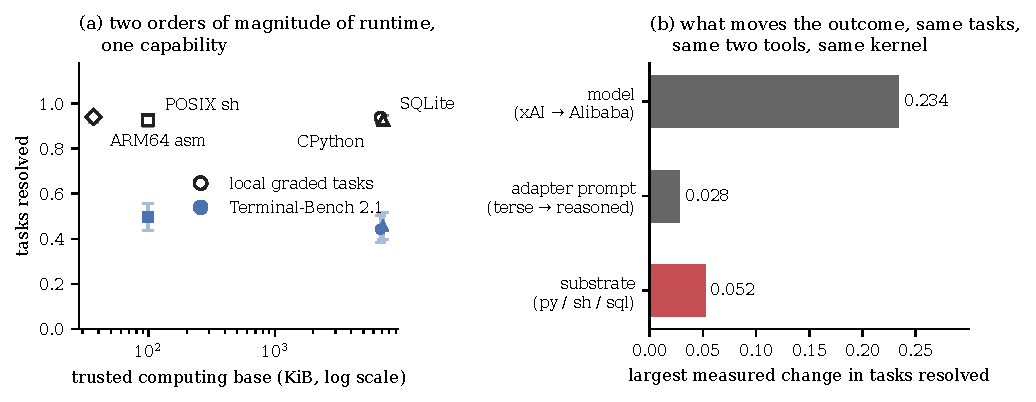
\includegraphics[width=\textwidth]{gen/fig-pareto}
\caption{The paper in one picture. \emph{(a)} Trusted computing base against
tasks resolved, for the local graded suite (all four substrates) and for
Terminal-Bench 2.1 (the three that run in a Linux container). The horizontal
axis spans two orders of magnitude; the vertical axis does not move with it.
Bars are Wilson intervals on the pooled trials, which are wider than the
task-paired intervals used for the equivalence verdicts and are shown here only
to keep the picture honest about sample size. \emph{(b)} The same outcome,
measured against the three things one can change while keeping the two
primitives and the specification fixed. Swapping the substrate is much the
smallest of the three, and the two that do move it are both on the model's side
of the boundary.}
\label{fig:pareto}
\end{figure}

\section{Terminal-Bench 2.1}
\label{sec:tb}

The suites so far are ours. This one is not: 89 container tasks with outcome
tests written by other people, run under Harbor with the official verifier.
The protocol was fixed in advance (\S\ref{sec:notrun}): dataset checkout
\texttt{7131e43}, 80 agent steps, the same two primitives, the same prompt
bytes, three repeats, and the three container-capable substrates run as three
concurrent jobs so that each sees the same slice of wall clock and the same
endpoint conditions.

Three models appear in this section and the reason is worth stating plainly.
The first arm ran on \texttt{deepseek-v4-flash} and was retired after 1560
trials because it was costing real money on a metered endpoint; the replacement
is served by a local relay at no per-token charge. That is a budget decision,
not a scientific one, and it costs comparability---so the retired arm is
reported rather than overwritten. The third arm is a single substrate on
\texttt{qwen3.8-max} from a different vendor, and exists only to put a number
on the model factor (\S\ref{sec:h3}).

\begin{table}[h]\centering\small
\caption{The arms. Protocols belong to the adapter, never to the kernel:
\texttt{a} forbids commentary, \texttt{b} requires a thought before the action,
\texttt{br} is \texttt{b} with an output budget wide enough for a model that
reasons before it answers.}
\label{tab:tbarms}
\widetable{gen/tab-tb-arms}
\end{table}

\begin{table}[h]\centering\small
\caption{\tbtrials\ trials: \tbtasks\ tasks $\times$ 3 substrates $\times$
\tbreps\ repeats. Rates are over scored trials.}
\label{tab:tb}
\begin{tabular}{lrrrrrr}
\toprule
substrate & rep 0 & rep 1 & rep 2 & all & resolved & pass$^3$ \\
\midrule
\texttt{py} & 0.461 & 0.483 & 0.384 & \textbf{0.443} & 116/262 & 0.286 \\
\texttt{sh} & 0.477 & 0.471 & 0.539 & \textbf{0.496} & 131/264 & 0.360 \\
\texttt{sql} & 0.494 & 0.404 & 0.471 & \textbf{0.457} & 121/265 & 0.345 \\
\bottomrule
\end{tabular}

\end{table}

\paragraph{What was excluded, and why it matters.}
Two kinds of failure end up in the same result file and must not be pooled.
An agent that runs out of wall clock has failed, and is scored~0. An
environment that will not build has not told us anything about the agent, and
is dropped. \tbexcluded\ trials were dropped and \tbagentfault\ were scored~0
under that rule (Table~\ref{tab:tbexclusions}); \tbexcludedfirstrep\ of the
exclusions land in repeat~0, nearly all of them \texttt{docker compose}
failures while the host pulled 60\,GB of task images for the first time. That
is a reason to report repeats separately rather than to average them away, and
it is the kind of accounting that decides whether a substrate looks worse
because it is worse or because its first pass ran during an image storm.

\begin{table}[h]\centering\small
\caption{Disposition of the trials that did not simply pass or fail.}
\label{tab:tbexclusions}
\begin{tabular}{llr}
\toprule
disposition & outcome & trials \\
\midrule
excluded & \texttt{VerifierTimeoutError} & 8 \\
excluded & \texttt{no\_reward} & 2 \\
scored 0 & \texttt{AgentTimeoutError} & 22 \\
scored 0 & \texttt{NonZeroAgentExitCodeError} & 1 \\
\bottomrule
\end{tabular}

\end{table}

\begin{table}[h]\centering\small
\caption{Pairwise equivalence on Terminal-Bench, paired by task, pooled over
repeats, 10{,}000-resample cluster bootstrap, pre-registered $\pm5$\,pp band.}
\label{tab:tbequiv}
\begin{tabular}{llrrrlll}
\toprule
A & B & rate A & rate B & diff & 95\% CI & verdict & p (Holm) \\
\midrule
\texttt{py} & \texttt{sh} & 0.440 & 0.493 & -0.052 & [-0.105, -0.004] & inconclusive & 0.355 \\
\texttt{py} & \texttt{sql} & 0.440 & 0.455 & -0.015 & [-0.073, +0.045] & inconclusive & 1 \\
\texttt{sh} & \texttt{sql} & 0.493 & 0.455 & +0.037 & [-0.011, +0.086] & inconclusive & 0.359 \\
\bottomrule
\end{tabular}

\end{table}

\begin{table}[h]\centering\small
\caption{The same substrate differences, one repeat at a time. A difference
that is real should persist across repeats; one that lives in a single repeat
is the model being unstable on hard tasks.}
\label{tab:tbperrep}
\begin{tabular}{lrrr}
\toprule
repeat & py $-$ sh & py $-$ sql & sh $-$ sql \\
\midrule
0 & -0.017 & -0.034 & -0.017 \\
1 & +0.011 & +0.078 & +0.067 \\
2 & -0.156 & -0.088 & +0.068 \\
\bottomrule
\end{tabular}

\end{table}

\paragraph{The result, stated as it came out.}
Of the three pairs, \tbequiv\ are \emph{equivalent}, \tbinconclusive\ are
\emph{inconclusive}, and \tbdifferent\ is \emph{different}. The largest point
difference is \tbmaxdiff, and its interval reaches just past the band, so the
pre-registered rule does not let us certify equivalence. McNemar finds no
significant difference on any pair (smallest Holm-adjusted $p$ is 0.36).

That largest difference deserves its own sentence, because it would be easy to
present it either as nothing or as a finding. It is \texttt{py} against
\texttt{sh}, and Table~\ref{tab:tbperrep} shows where it comes from: the first
two repeats put the two substrates within 0.017 of each other and disagree
about which is ahead, and the whole of the pooled difference comes from the
third. The 28 tasks the two disagree on split in both directions with no
pattern. We read that as a single repeat's luck at a base rate near 0.5, where
per-task variance is at its maximum---but we report the pooled number, the
per-repeat decomposition and the non-significant test, and leave the reader to
disagree.

So the honest summary is: no evidence of a substrate effect on any pair, and
not enough resolution to certify its absence at $\pm5$\,pp on this benchmark at
this sample size.

That the intervals are wide is not a defect of the design so much as a
property of the operating point. The substrates disagree on \tbdisagree\ of
\tbtasks\ tasks, always by one or two repeats out of three and in both
directions, with nothing concentrated on any substrate---the signature of a
model that is unstable on hard tasks rather than of a runtime that is worse.
Only \tbeveryone\ tasks are solved by every substrate on every repeat, and only
\tbsomeone\ are solved by anything at all: with a two-primitive kernel, no
exam-style delivery prompting, and this model, most of Terminal-Bench 2.1 is
out of reach, and a low base rate with high per-task variance is exactly the
regime in which $\pm5$\,pp is expensive to certify.

\paragraph{What moved the absolute rate.}
Between the first arm and the second the resolved rate went from \tbarmone\ to
\tbarmtwo. Every step of that came from the adapter or the model; the kernels,
the ABI and the two primitives were untouched, and the substrate verdicts are
unaffected because all three substrates always share one adapter, byte for
byte.

Most of the change has a single identifiable cause, and it is a result about
prompt design rather than a defect report. Protocol \texttt{a} instructed the
model to emit an action and nothing else, and the model ran with reasoning
disabled. Between them, those two choices leave the model no channel in which
to notice that its last command failed---so it re-issues it. In one measured
run, 25 actions contained 9 distinct commands, one of them repeated verbatim
ten times. Across the arm the median run spent 80 of its 80 steps and halted
voluntarily 12\% of the time. Protocol \texttt{b} changes one thing, requiring
a short thought before the action, and the median falls to 15 steps with
voluntary halts at 36\%.\footnote{Two integration details cost us runs and are
recorded here for anyone wiring a reasoning model into a tool loop rather than
as findings. First, \texttt{max\_tokens} covers reasoning tokens: a model can
spend the whole allowance thinking and return empty content, which an adapter
should not score as a protocol error. Second, a container cannot reach a relay
on the host's loopback address; rewriting the model URL for that case must not
also rewrite it for an endpoint on the public internet. The second cost a whole
pilot, which died after one step per trial with three transport errors and a
clean abort---the kernel doing exactly what \S\ref{sec:alm} says while the
adapter fed it a broken URL.}

The interesting part is the size of the correction relative to what it did not
fix. Removing the loop is worth \tbpromptdiff\ on the same 89 tasks: real, and
an order of magnitude less than the gap to a mature harness. The loop was
burning steps that were not going to solve those tasks anyway.

Two ways to sharpen the substrate verdicts exist and both are honest: more
repeats, which narrows the interval without changing the design, or a stronger
model, which raises the base rate. We report the pre-registered three repeats
rather than adding data until a verdict appears.

\section{Reliability}
\label{sec:faults}

Capability is not the only thing a runtime is for. We corrupt four channels at
the same rate $\lambda$: the model returns unparsable output, the model call
fails in transport, the tool fails or times out, and every event is redelivered
with probability $\lambda$. The policy is held fixed, so what moves is the
runtime's problem.

\begin{table}[h]\centering\small
\caption{Fault surface. \texttt{no\_repair}, \texttt{no\_retry} and
\texttt{no\_recovery} remove the corresponding budgets from the kernel.}
\label{tab:faults}
\begin{tabular}{lrrrrrr}
\toprule
arm & $\lambda$ & runs & success & model calls/run & redelivered/run & duplicate effects \\
\midrule
\texttt{full} & 0.0 & 800 & 1.000 & 3.52 & 0.00 & 0 \\
\texttt{full} & 0.01 & 800 & 1.000 & 3.64 & 0.06 & 0 \\
\texttt{full} & 0.05 & 800 & 1.000 & 4.28 & 0.37 & 0 \\
\texttt{full} & 0.1 & 800 & 1.000 & 5.08 & 0.98 & 0 \\
\texttt{full} & 0.3 & 800 & 0.930 & 7.72 & 3.86 & 0 \\
\texttt{full} & 0.5 & 800 & 0.520 & 7.96 & 5.89 & 0 \\
\texttt{no\_recovery} & 0.0 & 800 & 1.000 & 3.52 & 0.00 & 0 \\
\texttt{no\_recovery} & 0.1 & 800 & 0.720 & 3.12 & 0.56 & 0 \\
\texttt{no\_recovery} & 0.3 & 800 & 0.305 & 2.48 & 1.05 & 0 \\
\texttt{no\_repair} & 0.0 & 800 & 1.000 & 3.52 & 0.00 & 0 \\
\texttt{no\_repair} & 0.1 & 800 & 0.850 & 3.63 & 0.64 & 0 \\
\texttt{no\_repair} & 0.3 & 800 & 0.505 & 3.60 & 1.64 & 0 \\
\texttt{no\_retry} & 0.0 & 800 & 1.000 & 3.52 & 0.00 & 0 \\
\texttt{no\_retry} & 0.1 & 800 & 0.840 & 4.21 & 0.78 & 0 \\
\texttt{no\_retry} & 0.3 & 800 & 0.515 & 4.30 & 2.04 & 0 \\
\bottomrule
\end{tabular}

\end{table}

Three results. First, bounded repair and retry buy \emph{nothing} in a clean
world (\fullclean\ against \norecclean\ at $\lambda=0$) and
$+\recoverygain$\,pp at $\lambda=0.10$ (\fullten\ against \norecten). Second, dropping them makes runs
\emph{cheaper} in model calls, because a run that aborts early spends fewer:
the wrong way to read a cost table, and a good illustration of why efficiency
numbers without an outcome column are misleading. Third, across the sweep
\faultredelivered\ events were redelivered and \faultdup\ produced a duplicate
side effect, on every substrate---absorbing redelivery is a property of the
specification, not of one implementation.

At $\lambda=0.5$ the full arm falls to \fullfifty. The core's error handling is
bounded on purpose; it converts an unreliable world into a slower one up to a
point, and then reports \texttt{protocol\_exhausted} rather than pretending.

\section{Systems}
\label{sec:systems}

\begin{table}[h]\centering\small
\caption{Footprint and performance. \emph{TCB} is the interpreter or binary,
every library it links, and---for the Python-backed kernels---exactly the
standard-library modules they import, not the whole install. Libraries in the
macOS dyld shared cache have no file on disk and count as zero, so \texttt{sh}
and \texttt{asm} are understated by libSystem.}
\label{tab:systems}
\widetable{gen/tab-systems}
\end{table}

``Cold'' is the first invocation of a run, whose pages, dynamic-linker caches
and (for the relational kernel) schema are not yet warm; ``warm p50'' is the
median of the remaining 199. The gap is a few milliseconds and matters only for
one-shot use.

Two sizes are reported for every kernel and both belong in any honest account.
Quoting kernel-only bytes alone is how an assembly kernel becomes ``a 9\,KB
agent'' while a JSON parser and libc sit underneath it; quoting only the TCB
hides the thing the paper is about. Lines of code appear last and with a
warning: one line of SQL, shell and assembly are not the same unit. The
substrate-independent complexity numbers are \almrules\ transition rules and
\almfields\ mutable control-state fields, fixed by the specification and
implemented in full by each kernel.

\begin{table}[h]\centering\small
\caption{Where the wall clock and the tokens go. $T_{orch}$ is everything that
is neither the model call nor the tool: prompt rendering, the ABI round trip,
and the kernel.}
\label{tab:cost}
\widetable{gen/tab-cost}
\end{table}

Figure~\ref{fig:pareto} puts the two sizes and the outcomes on one plot.
The four kernels span \throughputspread$\times$ in transition throughput, and
that spread is almost invisible end to end: the slowest kernel costs
\slowestus\,$\mu$s per transition, or \slowestshare\% of a 500\,ms model call,
and measured orchestration time is \orchshare\ of wall clock across every
live run in this paper, against \modelshare\ spent waiting for the model.
This is the quantitative form of the paper's central negative result.
Orchestration substrate is operationally necessary---something has to hold the
budget, the phase and the idempotency---and it is no longer where the time
goes.

\section{Relation to a production runtime}
\label{sec:seed}

The kernels above are research instruments. The same repository contains a
production agent, \texttt{seed.sh}: a single POSIX shell file with a capability
index, prompt packs, skills, a memory lifecycle, delegation and run evidence.
It is roughly $10^5$ bytes, and it is \emph{not} evidence for anything in
\S\S\ref{sec:h1}--\ref{sec:systems}. We keep the two apart because conflating
them is the easiest way to make a minimality claim that is not true: a file
with a memory system is not a minimal core, whatever language it is in.

For context, and with the caveats stated where the numbers are: on the official
Terminal-Bench 2.1 suite (89 tasks, Harbor, official verifier, $k{=}1$, one
shared model) \texttt{seed.sh} resolved 45/89 (mean 0.506), against 66/89
(0.742) for mini-SWE-agent and 62/89 (0.697) for Terminus-2 under the same
model and harness. The gap is concentrated in \texttt{AgentTimeoutError}
(32 versus 12 and 11), not in a collapse of correctness among work that reached
the verifier, and the install surfaces are not equal---mini-SWE-agent's Harbor
adapter is given a Python toolchain, while the Seed container is given curl and
CA certificates. That comparison is a systems report about a production agent
at $k{=}1$; it is not a leaderboard rank, and it is not a measurement of ALM.

\section{Limitations}

\begin{itemize}
\item The end-to-end task evidence is \localtasks\ local tasks and four witness
families, not a 89-task container benchmark. The Terminal-Bench matrix is
pre-registered and unrun (\S\ref{sec:notrun}); until it is run, H2 is
established on smaller and easier work than the community standard.
\item The model factor is one vendor pair, not a survey, and the two models
differ in speed as well as in ability, so part of the gap in
Table~\ref{tab:modelfactor} belongs to this benchmark's wall clock. Both limits
are shown in that table rather than folded away.
\item Three models were used across the study and they are not interchangeable:
the substrate verdicts come from one of them, and the arm that established them
first was retired mid-study on cost. Everything is reported per arm, but a
single arm carried on one model throughout would have been cleaner.
\item The largest single lesson here is negative and was expensive: 1275 trials
were paid for before a trace was read carefully enough to notice the agent was
re-issuing the same failed command. Cheap qualitative inspection should precede
expensive quantitative runs, and in this study it did not.
\item The witness families are designed to separate arms. They are evidence
about the core, not an estimate of how often real tasks need feedback.
\item The assembly kernel runs on macOS and Linux but only on arm64, and its
history ring holds 4096 entries.
\item The fault injector corrupts four channels with independent Bernoulli
draws. Real failures are correlated and bursty.
\item Everything here is single-agent and finite-horizon by construction.
\end{itemize}

\section{Pre-registration, and what is still not run}
\label{sec:notrun}

The Terminal-Bench protocol was fixed before any of it was run: frozen dataset
commit and per-task manifest, frozen decoding and budget parameters, a
$\pm5$\,pp equivalence band with the bootstrap and correction named in advance,
and a 30-task subset selected by $\mathrm{sha256}(\text{salt} \| \text{task})$
under proportional allocation by difficulty and written to disk before any
result existed. \S\ref{sec:tb} is that protocol executed on the primary model.

One deviation, declared: the pre-registration interleaves substrates inside
each task block; we instead ran the three substrates as three concurrent jobs,
which exposes them to the same wall clock and the same endpoint state more
tightly than block interleaving would.

Two deviations are on the record and neither was decided by looking at an
outcome. The first arm's amendment promised five repeats and was stopped after
four and 82\% of the fifth, on cost. One repeat of the second arm was discarded
and re-run after the host filled its disk mid-arm: that repeat recorded
seventeen infrastructure faults against the neighbouring repeat's four, and the
discarded directories are kept beside the replacements so the claim can be
checked. A single-substrate arm on a third model was discarded on the same
grounds, twenty-three faults against one.

Still unrun: the same-model external baselines, which bear on the production
runtime of \S\ref{sec:seed} rather than on any hypothesis here. The assembly
kernel is absent from the Terminal-Bench arm because those images are
linux/amd64.

\section{Conclusion}

Separating $\kappa$ from $\mu$ and $\varepsilon$, and forbidding $\kappa$ to
read payload bytes, leaves an agent loop small enough to write in assembly and
in SQL triggers, and precise enough that four such implementations agree on
every one of \confcases\ recorded cases, trace record by trace record. Holding
the model and the environment fixed, which of them runs the loop does not
measurably change what the agent accomplishes, while it changes the trusted
computing base by two orders of magnitude. What the core does buy is visible
elsewhere: feedback, cross-step state and the recursion are load-bearing for
capability, and bounded repair, retry and idempotency are load-bearing for
reliability---worth nothing in a clean world and \recoverygain\ points at a
10\% fault rate. The interesting question about agent runtimes is not how small they can
be made. It is which of their parts are paying for capability, which for
reliability, and which for neither.

\section*{Artifacts}

Specification, four kernels, conformance suite, witness families, statistics
and the generated result tables: \url{https://github.com/Leehow/seed} under
\texttt{alm/}. Every table in this paper is generated from a results file by
\texttt{alm/paper\_tables.py}; no number is transcribed by hand.

\appendix
\section{Rule coverage of the conformance suite}

\begin{table}[h]\centering\small
\caption{Every transition in the specification and how often the suite fires
it. Generated with the cases.}
\label{tab:coverage}
\begin{tabular}{llrr}
\toprule
rule & specification & trace records & cases \\
\midrule
\texttt{start} & s4.1 start & 350 & 350 \\
\texttt{tool} & s4.2 model calls a tool & 1195 & 317 \\
\texttt{halt} & s4.3 model halts & 204 & 204 \\
\texttt{halt\_disabled} & s8 halt refused (ext) & 23 & 13 \\
\texttt{repair} & s4.5 protocol repair & 62 & 45 \\
\texttt{abort\_protocol} & s4.5 repairs exhausted & 35 & 35 \\
\texttt{retry} & s4.5 transport retry & 23 & 18 \\
\texttt{abort\_transport} & s4.5 retries exhausted & 13 & 13 \\
\texttt{observe} & s4.4 observation, run continues & 1097 & 307 \\
\texttt{abort\_budget} & s4.4 budget exhausted & 98 & 98 \\
\texttt{stale\_event} & s4.6 event ignored & 384 & 50 \\
\texttt{after\_terminal} & s4.6 event after terminal & 102 & 50 \\
\bottomrule
\end{tabular}

\end{table}

\bibliographystyle{plain}
\bibliography{refs}

\end{document}
